
\chapter{Simple Derivatives}

\section{Derivatives of Matrices, Vectors and Scalar Forms}

\subsection{First Order}

The Matrix Cookbook defines the single-entry matrix $J^{i,j} \in R^{n\times n}$ as the matrix which is zero everywhere except in the entry $(i, j)$ in which it is 1.
Alternatively we could write $J^{i,j}_{n,m} = [i=n][j=m]$.

\begin{align*}
   \tag{69}
   \frac{\partial x^T a}{\partial x}
   &= \frac{\partial a^T x}{\partial x}
   = a
   &
      \begin{tikzpicture}[baseline=(a0.base), inner sep=1pt]
         \node (a0) {$(x$};
         \node[right=1em of a0] (a1) {$a)$};
         \path (a0) edge (a1);
         \draw [d] (a1.east) -- ++(.2,.2);
      \end{tikzpicture}
   &=
      \begin{tikzpicture}[baseline=(a0.base), inner sep=1pt]
         \node (a0) {$(x)$};
         \node[right=1em of a0] (a1) {$a$};
         \path (a0) edge (a1);
         \draw [d] (a0.east) -- ++(.2,.2);
      \end{tikzpicture}
   =
      \begin{tikzpicture}[baseline=(a0.base), inner sep=1pt]
         \node (a0) {};
         \node[right=1em of a0] (a1) {$a$};
         \path (a0) edge (a1);
         \draw (a0.east) -- ++(-.1,-.2);
      \end{tikzpicture}
   \\
   %%%%%%%%%%%%%%%%%%%%%%%%%%%%%%%%%%%%%%%%
   \tag{70}
   \frac{\partial a^T X b}{\partial X} &= ab^T
   &
      \begin{tikzpicture}[baseline=(a0.base), inner sep=1pt]
         \node (a0) {$(a$};
         \node[right=1em of a0] (a1) {$X$};
         \node[right=1em of a1] (a2) {$b)$};
         \path (a0) edge (a1);
         \path (a1) edge (a2);
         \draw[d] (a2.east) -- ++(.2,.2);
         \draw[d] (a2.east) -- ++(.3,.1);
      \end{tikzpicture}
   &=
      \begin{tikzpicture}[baseline=(a0.base), inner sep=1pt]
         \node (a0) {$a$};
         \node[right=1em of a0] (a1) {$(X)$};
         \node[right=1em of a1] (a2) {$b$};
         \path (a0) edge (a1);
         \path (a1) edge (a2);
         \draw[d] (a1.east) -- ++(.2,.2);
         \draw[d] (a1.east) -- ++(.3,.1);
      \end{tikzpicture}
      =
      \begin{tikzpicture}[baseline=(a0.base), inner sep=1pt]
         \node (a0) {$a$};
         \node[right=1em of a0] (a1) {};
         \node[right=1em of a1] (a2) {$b$};
         \path (a0) edge (a1);
         \path (a1) edge (a2);
         \draw (a1.west) -- ++(.1,.2);
         \draw (a1.east) -- ++(-.1,-.2);
      \end{tikzpicture}
   \\
   %%%%%%%%%%%%%%%%%%%%%%%%%%%%%%%%%%%%%%%%
   \tag{73}
   \frac{\partial X}{\partial X_{i,j}} &= J^{i,j}
   &
      \begin{tikzpicture}[baseline=(a0.base), inner sep=1pt]
         \node (a0) {$($};
         \node[right=1em of a0] (a1) {$X$};
         \node[right=1em of a1] (a2) {$)$};
         \path (a0) edge (a1);
         \path (a1) edge (a2);
         \draw[d] (a2.east) -- ++(.2,.2) node[midway, above left, font=\tiny] {i};
         \draw[d] (a2.east) -- ++(.3,.1) node[midway, below right, font=\tiny] {j};
      \end{tikzpicture}
   &=
      \begin{tikzpicture}[baseline=(a0.base), inner sep=1pt]
         \node (a0) {};
         \node[right=1em of a0] (a1) {};
         \node[right=1em of a1] (a2) {};
         \path (a0) edge (a1);
         \path (a1) edge (a2);
         \draw (a1.west) -- ++(.1,.2) node[midway, above left, font=\tiny] {i};
         \draw (a1.east) -- ++(-.1,-.2) node[midway, below right, font=\tiny] {j};
      \end{tikzpicture}
   \\
   %%%%%%%%%%%%%%%%%%%%%%%%%%%%%%%%%%%%%%%%
   \tag{74}
   \frac{\partial (X A)_{i,j}}{\partial X_{m,n}} &= (J^{m,n} A)_{i,j}
   &
      \begin{tikzpicture}[baseline=(a0.base), inner sep=1pt]
         \node (a0) {$($};
         \node[right=1em of a0] (a1) {$X$};
         \node[right=1em of a1] (a2) {$A$};
         \node[right=1em of a2] (a3) {$)$};
         \draw (a0) -- (a1) node[midway, above left, font=\tiny] {i};
         \draw (a1) -- (a2);
         \draw (a2) -- (a3) node[midway, below right, font=\tiny] {j};
         \draw[d] (a3.east) -- ++(.2,.2) node[midway, above left, font=\tiny] {m};
         \draw[d] (a3.east) -- ++(.3,.1) node[midway, below right, font=\tiny] {n};
      \end{tikzpicture}
   &=
      \begin{tikzpicture}[baseline=(a0.base), inner sep=1pt]
         \node (a0) {};
         \node[right=1em of a0] (a1) {$(X)$};
         \node[right=1em of a1] (a2) {$A$};
         \node[right=1em of a2] (a3) {};
         \path (a0) edge (a1);
         \path (a1) edge (a2);
         \path (a2) edge (a3);
         \draw[d] (a1.east) -- ++(.2,.2);
         \draw[d] (a1.east) -- ++(.3,.1);
      \end{tikzpicture}
 \\&&&=
      \begin{tikzpicture}[baseline=(a0.base), inner sep=1pt]
         \node (a0) {};
         \node[right=1em of a0] (a1) {};
         \node[right=1em of a1] (a2) {$A$};
         \node[right=1em of a2] (a3) {};
         \draw (a0) -- (a1) node[midway, above left, font=\tiny] {i};
         \draw (a1) -- (a2);
         \draw (a2) -- (a3) node[midway, below right, font=\tiny] {j};
         \draw (a1.west) -- ++(.1,.2) node[midway, above left, font=\tiny] {m};
         \draw (a1.east) -- ++(-.1,-.2) node[midway, below right, font=\tiny] {n};
      \end{tikzpicture}
\end{align*}

\subsection{Second Order}
\noindent
\makebox[\textwidth]{\parbox{1.1\textwidth}{%
\begin{align*}
   \tag{76}
   \frac{\partial}{\partial X_{i,j}}
   \sum_{k,l,m,n} X_{k,l} X_{m,n}
   &= (\sum_{k,l} X_{k,l})^2
   %&= \frac{\partial \|X\|_F^2}{\partial X_{i,j}}
   %&= 2\, \sum_{k,l} X_{k,l}
   &
   \begin{tikzpicture}[baseline=.5em, inner sep=1pt]
      \node (a0) at (0,0) {$\sbullet$};
      \node (a1) at (.5,0) {$X$};
      \node (a2) at (1,0) {$\sbullet$};
      \path (a0) edge (a1);
      \path (a1) edge (a2);
      \node (b0) at (0, .5) {$\sbullet$};
      \node (b1) at (.5, .5) {$X$};
      \node (b2) at (1, .5) {$\sbullet$};
      \path (b0) edge (b1);
      \path (b1) edge (b2);
      \node at (-.25, .25) {$\bigg($};
      \node at (1.25, .25) {$\bigg)$};
      \draw[d] (1.35, .4) -- ++(.2,.2) node[midway, above left, font=\tiny] {i};
      \draw[d] (1.35, .4) -- ++(.3,.1) node[midway, below right, font=\tiny] {j};
   \end{tikzpicture}
   &=
   \begin{tikzpicture}[baseline=.5em, inner sep=1pt]
      \node (a0) at (0,0) {$\sbullet$};
      \node (a1) at (.5,0) {$(X)$};
      \node (a2) at (1,0) {$\sbullet$};
      \path (a0) edge (a1);
      \path (a1) edge (a2);
      \node (b0) at (0, .5) {$\sbullet$};
      \node (b1) at (.5, .5) {$X$};
      \node (b2) at (1, .5) {$\sbullet$};
      \path (b0) edge (b1);
      \path (b1) edge (b2);
      \draw[d] (.83,.0) -- ++(.2,.2);
      \draw[d] (.83,.0) -- ++(.3,.1);
   \end{tikzpicture}
   +
   \begin{tikzpicture}[baseline=.5em, inner sep=1pt]
      \node (a0) at (0,0) {$\sbullet$};
      \node (a1) at (.5,0) {$X$};
      \node (a2) at (1,0) {$\sbullet$};
      \path (a0) edge (a1);
      \path (a1) edge (a2);
      \node (b0) at (0, .5) {$\sbullet$};
      \node (b1) at (.5, .5) {$(X)$};
      \node (b2) at (1, .5) {$\sbullet$};
      \path (b0) edge (b1);
      \path (b1) edge (b2);
      \draw[d] (0.83,.5) -- ++(.2,.2);
      \draw[d] (0.83,.5) -- ++(.3,.1);
   \end{tikzpicture}
   %\\[.3em]
   \\
   &= 2\, \sum_{k,l} X_{k,l}
   &&=
   2\,
   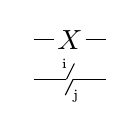
\begin{tikzpicture}[baseline=.5em, inner sep=1pt]
      \node (a0) at (0,0) {$\sbullet$};
      \node (a1) at (.5,0) {};
      \node (a2) at (1,0) {$\sbullet$};
      \path (a0) edge (a1);
      \path (a1) edge (a2);
      \node (b0) at (0, .5) {$\sbullet$};
      \node (b1) at (.5, .5) {$X$};
      \node (b2) at (1, .5) {$\sbullet$};
      \path (b0) edge (b1);
      \path (b1) edge (b2);
      \draw (a1.west) -- ++(.1,.2) node[midway, above left, font=\tiny] {i};
      \draw (a1.east) -- ++(-.1,-.2) node[midway, below right, font=\tiny] {j};
   \end{tikzpicture}
   %%%%%%%%%%%%%%%%%%%%%%%%%%%%%%%%%%%%%%%%
   \\[.5em]
   \tag{77} 
   \frac{\partial b^T X^T X c}{\partial X} &= X(bc^T + cb^T) 
   &
   \begin{tikzpicture}[baseline=(a0.base), inner sep=1pt]
      \node (a0) {$(\vecmatvec{.5em}{b}{X^T,X}{c})$};
      \draw[d] (a0.east) -- ++(.2,.2);
      \draw[d] (a0.east) -- ++(.3,.1);
   \end{tikzpicture}
   &=
   \begin{tikzpicture}[baseline=(a0.base), inner sep=1pt]
      \node (a0) {$b$};
      \node[right=1em of a0] (a1) {$X^T$};
      \node[right=1em of a1] (a2) {$(X)$};
      \node[right=1em of a2] (a3) {$c$};
      \draw (a0) -- (a1);
      \draw (a1) -- (a2);
      \draw (a2) -- (a3);
      \draw[d] (a2.east) -- ++(.2,.2);
      \draw[d] (a2.east) -- ++(.3,.1);
   \end{tikzpicture}
 \\&&&+
   \begin{tikzpicture}[baseline=(a0.base), inner sep=1pt]
      \node (a0) {$b$};
      \node[right=1em of a0] (a1) {$(X^T)$};
      \node[right=1em of a1] (a2) {$X$};
      \node[right=1em of a2] (a3) {$c$};
      \draw (a0) -- (a1);
      \draw (a1) -- (a2);
      \draw (a2) -- (a3);
      \draw[d] (a1.east) -- ++(.2,.2);
      \draw[d] (a1.east) -- ++(.3,.1);
   \end{tikzpicture}
   \\[.3em]&&&=
   \begin{tikzpicture}[baseline=(a0.base), inner sep=1pt]
      \node (a0) {$b$};
      \node[right=1em of a0] (a1) {$X^T$};
      \node[right=1em of a1] (a2) {};
      \node[right=1em of a2] (a3) {$c$};
      \draw (a0) -- (a1);
      \draw (a1) -- (a2);
      \draw (a2) -- (a3);
      \draw (a2.west) -- ++(.1,.2);
      \draw (a2.east) -- ++(-.1,-.2);
   \end{tikzpicture}
 \\&&&+
   \begin{tikzpicture}[baseline=(a0.base), inner sep=1pt]
      \node (a0) {$b$};
      \node[right=1em of a0] (a1) {};
      \node[right=1em of a1] (a2) {$X$};
      \node[right=1em of a2] (a3) {$c$};
      \draw (a0) -- (a1);
      \draw (a1) -- (a2);
      \draw (a2) -- (a3);
      \draw (a1.west) -- ++(.1,.2);
      \draw (a1.east) -- ++(-.1,-.2);
   \end{tikzpicture}
   \\[.3em]&&&=
   \begin{tikzpicture}[baseline=(a0.base), inner sep=1pt]
      \node (a0) {$X$};
      \node[right=.7em of a0] (a1) {$($};
      \node[right=.4em of a1] (a2) {$b\, c$};
      \node[right=.4em of a2] (a4) {$+$};
      \node[right=.6em of a4] (a5) {$c\, b$};
      \node[right=.2em of a5] (a7) {$)$};
      \draw (a0.west) -- ++(-.2,0);
      \draw (a0) -- (a1);
      \draw (a2.west) -- ++(-.2,0);
      \draw (a2.east) -- ++(.1,.15);
      \draw (a5.west) -- ++(-.2,0);
      \draw (a5.east) -- ++(.1,.15);
   \end{tikzpicture}
   \\
   \tag{78} 
   \frac{\partial}{\partial x} (Bx+b)^T C (Dx+d) &= B^TC(Dx+d)&&
                                \\&+D^TC^T(Bx+b) 
   &
   \dots &
   \\
   \tag{79} 
   \frac{\partial}{\partial X_{i,j}} (X^TBX)_{k,l} &= \delta_{l,j}(X^TB)_{k,i}
   %  \\&+ \delta_{k,j}(BX)_{i,l} 
   &
   \begin{tikzpicture}[baseline=(a0.base), inner sep=1pt]
      \node (a0) {$($};
      \node[right=.5em of a0] (a1) {$X^T$};
      \node[right=.5em of a1] (a2) {$B$};
      \node[right=.5em of a2] (a3) {$X$};
      \node[right=.5em of a3] (a4) {$)$};
      \draw (a0) -- (a1) node[midway, above left, font=\tiny] {k};
      \draw (a1) -- (a2);
      \draw (a2) -- (a3);
      \draw (a3) -- (a4) node[midway, below right, font=\tiny] {l};
      \draw[d] (a4.east) -- ++(.2,.2) node[midway, above left, font=\tiny] {i};
      \draw[d] (a4.east) -- ++(.3,.1) node[midway, below right, font=\tiny] {j};
   \end{tikzpicture}
   &=
   \begin{tikzpicture}[baseline=(a0.base), inner sep=1pt]
      \node (a0) {};
      \node[right=.5em of a0] (a1) {$X^T$};
      \node[right=.5em of a1] (a2) {$B$};
      \node[right=.5em of a2] (a3) {};
      \node[right=.5em of a3] (a4) {};
      \draw (a0) -- (a1) node[midway, above left, font=\tiny] {k};
      \draw (a1) -- (a2);
      \draw (a2) -- (a3);
      \draw (a3) -- (a4) node[midway, below right, font=\tiny] {l};
      \draw (a3.west) -- ++(.1,.2) node[midway, above left, font=\tiny] {i};
      \draw (a3.east) -- ++(-.1,-.2) node[midway, below right, font=\tiny] {j};
   \end{tikzpicture}
   \\
   &+ \delta_{k,j}(BX)_{i,l}
   &&+
   \begin{tikzpicture}[baseline=(a0.base), inner sep=1pt]
      \node (a0) {};
      \node[right=.5em of a0] (a1) {};
      \node[right=.5em of a1] (a2) {$B$};
      \node[right=.5em of a2] (a3) {$X$};
      \node[right=.5em of a3] (a4) {};
      \draw (a0) -- (a1) node[midway, above left, font=\tiny] {k};
      \draw (a1) -- (a2);
      \draw (a2) -- (a3);
      \draw (a3) -- (a4) node[midway, below right, font=\tiny] {l};
      \draw (a1.west) -- ++(.1,.2) node[midway, above left, font=\tiny] {j};
      \draw (a1.east) -- ++(-.1,-.2) node[midway, below right, font=\tiny] {i};
   \end{tikzpicture}
   %%%%%%%%%%%%%%%%%%%%%%%%%%%%%%%%%%%%%%%%
   \\
   \tag{80} 
   \frac{\partial}{\partial X_{i,j}} X^TBX &= X^TBJ^{i,j} + J^{j,i}BX 
   &
   \text{(same as above)} &
   %%%%%%%%%%%%%%%%%%%%%%%%%%%%%%%%%%%%%%%%
   \\
   \tag{81} 
   \frac{\partial}{\partial x} x^TBx &= (B+B^T)x 
   &
   \begin{tikzpicture}[baseline=(a0.base), inner sep=1pt]
      \node (a0) {$(x$};
      \node[right=.5em of a0] (a1) {$B$};
      \node[right=.5em of a1] (a2) {$x)$};
      \draw (a0) -- (a1);
      \draw (a1) -- (a2);
      \draw[d] (a2.east) -- ++(.2,.2) node[midway, above left, font=\tiny] {i};
      \draw[d] (a2.east) -- ++(.3,.1) node[midway, below right, font=\tiny] {j};
   \end{tikzpicture}
   &=
   \vecmatvec{.5em}{}{B}{x}
   + \vecmatvec{.5em}{x}{B}{}
 \\&&&=
   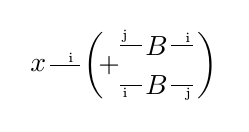
\begin{tikzpicture}[baseline=.5em, inner sep=1pt]
      \node (a0) at (0,0) {};
      \node (a1) at (.5,0) {$B$};
      \node (a2) at (1,0) {};
      \draw (a0) -- (a1) node[midway, below left, font=\tiny] {i};
      \draw (a1) -- (a2) node[midway, below right, font=\tiny] {j};
      \node (b0) at (0, .5) {};
      \node (b1) at (.5, .5) {$B$};
      \node (b2) at (1, .5) {};
      \draw (b0) -- (b1) node[midway, above left, font=\tiny] {j};
      \draw (b1) -- (b2) node[midway, above right, font=\tiny] {i};
      \node (l) at (-.3, .25) {$\bigg($};
      \node at (1.15, .25) {$\bigg)$};
      \node at (-.1, .25) {$+$};
      \node (x) at (-1,.25) {$x$};
      \draw (x) -- (l) node[midway, above right, font=\tiny] {i};
   \end{tikzpicture}
   %%%%%%%%%%%%%%%%%%%%%%%%%%%%%%%%%%%%%%%%
   \\
   \tag{82} 
   \frac{\partial}{\partial X} b^T X^T D X c &= D^T X b c^T + DXcb^T 
   &
   \dots &
   \\
   \tag{83} 
   \frac{\partial}{\partial X} (Xb+c)^T D (Xb+c) &= (D+D^T)(Xb+c)b^T 
   &
   \dots &
   \\
\end{align*}
}}

Assume $W$ is symmetric, then... (84) - (88)

\subsection{Higher-order and non-linear}


$$
\frac{\partial\left(\mathbf{X}^n\right)_{k l}}{\partial X_{i j}}=\sum_{r=0}^{n-1}\left(\mathbf{X}^r \mathbf{J}^{i j} \mathbf{X}^{n-1-r}\right)_{k l}
$$

For proof of the above, see B.1.3.
$$
\frac{\partial}{\partial \mathbf{X}} \mathbf{a}^T \mathbf{X}^n \mathbf{b}=\sum_{r=0}^{n-1}\left(\mathbf{X}^r\right)^T \mathbf{a b}^T\left(\mathbf{X}^{n-1-r}\right)^T
$$

\section{Derivatives of Traces}
Assume F(X) to be a differentiable function of each of the elements of X. It
then holds that
\[\frac{d \mathrm{Tr}(F(x))}{dX} = f(X)^T,\]
where $f(\cdot)$ is the scalar derivative of $F(\cdot)$.

TODO: To show this with tensor diagrams, we first need to introduce our notation for functions.

% Many more examples here: https://mbustamanter.github.io/ssg-blog/matder1/

\subsection{First Order}

\begin{align*}
   \tag{99}
   \frac{\partial}{\partial X} \mathrm{Tr}(X)
   &= I
   &
   \hspace{-1em}
   \begin{tikzpicture}[baseline=(a0.base), inner sep=1pt]
      \node (a0) {$($};
      \node[right=1em of a0] (a1) {$X$};
      \node[right=1em of a1] (a3) {$)$};
      \path (a1) edge[out=160, in=20, loop] (a1);
      \draw[d] (a3.east) -- ++(.2,.2);
      \draw[d] (a3.east) -- ++(.3,.1);
   \end{tikzpicture}
   \hspace{-1em}
   &=
   \hspace{-2em}
   \begin{tikzpicture}[baseline=(a0.base), inner sep=1pt]
      \node (a1) {$(X)$};
      \path (a1) edge[out=160, in=20, loop, looseness=4] (a1);
      \draw[d] (a1.south east) -- ++(.2,-.2);
      \draw[d] (a1.south east) -- ++(.3,-.1);
   \end{tikzpicture}
   \hspace{-2em}
 \\&&&=
   \hspace{-1.5em}
   \begin{tikzpicture}[baseline=(a0.base), inner sep=1pt]
      \node (a1) {$\phantom{X}$};
      \path (a1) edge[out=160, in=20, loop, looseness=6] (a1);
      \draw ($(a1.east)-(0,-.2em)$) -- ++(.2,-.1);
      \draw ($(a1.west)-(0,-.2em)$) -- ++(-.2,-.1);
   \end{tikzpicture}
   \hspace{-1.5em}
 \\&&&=
   \matmul{\sbullet}
   %%%%%%%%%%%%%%%%%%%%%%%%%%%%%%
   \\
   \tag{100}
   \frac{\partial}{\partial X} \mathrm{Tr}(XA)
   &= A^T
   &
   \begin{tikzpicture}[baseline=(a0.base), inner sep=1pt]
      \node (a0) {$($};
      \node[right=1em of a0] (a1) {$X$};
      \node[right=1em of a1] (a2) {$A$};
      \node[right=1em of a2] (a3) {$)$};
      \draw (a1) -- (a2);
      \path (a1) edge[out=160, in=20, looseness=2] (a2);
      \draw[d] (a3.east) -- ++(.2,.2);
      \draw[d] (a3.east) -- ++(.3,.1);
   \end{tikzpicture}
   &=
   \hspace{-2em}
   \begin{tikzpicture}[baseline=(a0.base), inner sep=1pt]
      \node (a1) {$(X)$};
      \node[right=1em of a1] (a2) {$A$};
      \draw (a1) -- (a2);
      \path (a1) edge[out=160, in=20, looseness=2] (a2);
      \draw[d] (a1.south east) -- ++(.2,-.2);
      \draw[d] (a1.south east) -- ++(.3,-.1);
   \end{tikzpicture}
   \hspace{-2em}
 \\&&&
   \hspace{-1.5em}
   \begin{tikzpicture}[baseline=(a0.base), inner sep=1pt]
      \node (a1) {$\phantom{X}$};
      \node[right=1em of a1] (a2) {$A$};
      \draw (a1) -- (a2);
      \path (a1) edge[out=160, in=20, looseness=2] (a2);
      \draw (a1.east) -- ++(.2,-.1);
      \draw ($(a1.west)-(0,-.2em)$) -- ++(-.2,-.1);
   \end{tikzpicture}
   \hspace{-1.5em}
 \\&&&
   = \matmul{A^T}
   %%%%%%%%%%%%%%%%%%%%%%%%%%%%%%
   \\
   \tag{101}
   \frac{\partial}{\partial X} \mathrm{Tr}(AXB)
   &= A^TB^T
   &
   \hspace{-1em}
   \begin{tikzpicture}[baseline=(a0.base), inner sep=1pt]
      \node (a0) {$($};
      \node[right=1em of a0] (a1) {$A$};
      \node[right=1em of a1] (a2) {$X$};
      \node[right=1em of a2] (a3) {$B$};
      \node[right=1em of a3] (a4) {$)$};
      \draw (a1) -- (a2) -- (a3);
      \path (a1) edge[out=160, in=20, looseness=2] (a3);
      \draw[d] (a4.east) -- ++(.2,.2);
      \draw[d] (a4.east) -- ++(.3,.1);
   \end{tikzpicture}
   \hspace{-1em}
   &=
   \hspace{-3em}
   \begin{tikzpicture}[baseline=(a0.base), inner sep=1pt]
      \node (a1) {$A$};
      \node[right=1em of a1] (a2) {$(X)$};
      \node[right=1em of a2] (a3) {$B$};
      \draw (a1) -- (a2) -- (a3);
      \path (a1) edge[out=160, in=20, looseness=2] (a3);
      \draw[d] (a2.south east) -- ++(.2,-.2);
      \draw[d] (a2.south east) -- ++(.3,-.1);
   \end{tikzpicture}
   \hspace{-3em}
 \\&&&=
   \hspace{-2.5em}
   \begin{tikzpicture}[baseline=(a0.base), inner sep=1pt]
      \node (a1) {$A$};
      \node[right=1em of a1] (a2) {$\phantom{X}$};
      \node[right=1em of a2] (a3) {$B$};
      \draw (a1) -- (a2) -- (a3);
      \path (a1) edge[out=160, in=20, looseness=2] (a3);
      \draw (a2.east) -- ++(.2,-.1);
      \draw (a2.west) -- ++(-.2,-.1);
   \end{tikzpicture}
   \hspace{-2.5em}
 \\&&&=
   \matmul{A^T, B^T}
\end{align*}


Continues for (102-105).
The last one uses the Kronecker product, which we may have to introduce first.

\subsection{Second Order}
\begin{align*}
   \frac{\partial}{\partial X} \mathrm{Tr}(X^2)
   &=2 X^T
   &
   \begin{tikzpicture}[baseline=(a0.base), inner sep=1pt]
      \node (a0) {$($};
      \node[right=1em of a0] (a1) {$X$};
      \node[right=1em of a1] (a2) {$X$};
      \node[right=1em of a2] (a3) {$)$};
      \draw (a1) -- (a2);
      \path (a1) edge[out=160, in=20, looseness=2] (a2);
      \draw[d] (a3.east) -- ++(.2,.2);
      \draw[d] (a3.east) -- ++(.3,.1);
   \end{tikzpicture}
   &=
   \hspace{-2em}
   \begin{tikzpicture}[baseline=(a0.base), inner sep=1pt]
      \node (a1) {$(X)$};
      \node[right=1em of a1] (a2) {$X$};
      \draw (a1) -- (a2);
      \path (a1) edge[out=160, in=20, looseness=2] (a2);
      \draw[d] (a1.south east) -- ++(.2,-.2);
      \draw[d] (a1.south east) -- ++(.3,-.1);
   \end{tikzpicture}
   \hspace{-2em}
   +
   \hspace{-2em}
   \begin{tikzpicture}[baseline=(a0.base), inner sep=1pt]
      \node (a1) {$X$};
      \node[right=1em of a1] (a2) {$(X)$};
      \draw (a1) -- (a2);
      \path (a1) edge[out=160, in=20, looseness=2] (a2);
      \draw[d] (a2.south east) -- ++(.2,-.2);
      \draw[d] (a2.south east) -- ++(.3,-.1);
   \end{tikzpicture}
   \hspace{-2em}
 \\&&&=
   \hspace{-1.5em}
   \begin{tikzpicture}[baseline=(a0.base), inner sep=1pt]
      \node (a1) {$\phantom{X}$};
      \node[right=1em of a1] (a2) {$X$};
      \draw (a1) -- (a2);
      \path (a1) edge[out=160, in=20, looseness=2] (a2);
      \draw (a1.east) -- ++(.2,-.1);
      \draw ($(a1.west)-(0,-.2em)$) -- ++(-.2,-.1);
   \end{tikzpicture}
   \hspace{-1.5em}
   +
   \hspace{-1.5em}
   \begin{tikzpicture}[baseline=(a0.base), inner sep=1pt]
      \node (a1) {$X$};
      \node[right=1em of a1] (a2) {$\phantom{X}$};
      \draw (a1) -- (a2);
      \path (a1) edge[out=160, in=20, looseness=2] (a2);
      \draw (a2.west) -- ++(-.2,-.1);
      \draw ($(a2.east)-(0,-.2em)$) -- ++(.2,-.1);
   \end{tikzpicture}
   \hspace{-1.5em}
 \\&&&=
   2\matmul{X^T}
\end{align*}
More:
\begin{align*}
& \frac{\partial}{\partial \mathbf{X}} \operatorname{Tr}\left(\mathbf{X}^2 \mathbf{B}\right)=(\mathbf{X B}+\mathbf{B X})^T \\
& \frac{\partial}{\partial \mathbf{X}} \operatorname{Tr}\left(\mathbf{X}^T \mathbf{B} \mathbf{X}\right)=\mathbf{B} \mathbf{X}+\mathbf{B}^T \mathbf{X} \\
& \frac{\partial}{\partial \mathbf{X}} \operatorname{Tr}\left(\mathbf{B} \mathbf{X} \mathbf{X}^T\right)=\mathbf{B} \mathbf{X}+\mathbf{B}^T \mathbf{X} \\
& \frac{\partial}{\partial \mathbf{X}} \operatorname{Tr}\left(\mathbf{X} \mathbf{X}^T \mathbf{B}\right)=\mathbf{B} \mathbf{X}+\mathbf{B}^T \mathbf{X} \\
& \frac{\partial}{\partial \mathbf{X}} \operatorname{Tr}\left(\mathbf{X B} \mathbf{X}^T\right)=\mathbf{X} \mathbf{B}^T+\mathbf{X B} \\
& \frac{\partial}{\partial \mathbf{X}} \operatorname{Tr}\left(\mathbf{B} \mathbf{X}^T \mathbf{X}\right)=\mathbf{X} \mathbf{B}^T+\mathbf{X B} \\
& \frac{\partial}{\partial \mathbf{X}} \operatorname{Tr}\left(\mathbf{X}^T \mathbf{X B}\right)=\mathbf{X} \mathbf{B}^T+\mathbf{X B} \\
& \frac{\partial}{\partial \mathbf{X}} \operatorname{Tr}(\mathbf{A X B X})=\mathbf{A}^T \mathbf{X}^T \mathbf{B}^T+\mathbf{B}^T \mathbf{X}^T \mathbf{A}^T \\
& \frac{\partial}{\partial \mathbf{X}} \operatorname{Tr}\left(\mathbf{X}^T \mathbf{X}\right)=\frac{\partial}{\partial \mathbf{X}} \operatorname{Tr}\left(\mathbf{X} \mathbf{X}^T\right)=2 \mathbf{X} \\
& \frac{\partial}{\partial \mathbf{X}} \operatorname{Tr}\left(\mathbf{B}^T \mathbf{X}^T \mathbf{C X B}\right)=\mathbf{C}^T \mathbf{X} \mathbf{B B}^T+\mathbf{C X B B}^T \\
& \frac{\partial}{\partial \mathbf{X}} \operatorname{Tr}\left[\mathbf{X}^T \mathbf{B X C}\right]=\mathbf{B X C}+\mathbf{B}^T \mathbf{X} \mathbf{C}^T \\
& \frac{\partial}{\partial \mathbf{X}} \operatorname{Tr}\left(\mathbf{A X B} \mathbf{X}^T \mathbf{C}\right)=\mathbf{A}^T \mathbf{C}^T \mathbf{X B}^T+\mathbf{C A X B} \\
& \frac{\partial}{\partial \mathbf{X}} \operatorname{Tr}\left[(\mathbf{A X B}+\mathbf{C})(\mathbf{A X B}+\mathbf{C})^T\right]=2 \mathbf{A}^T(\mathbf{A X B}+\mathbf{C}) \mathbf{B}^T \\
& \frac{\partial}{\partial \mathbf{X}} \operatorname{Tr}(\mathbf{X} \otimes \mathbf{X})=\frac{\partial}{\partial \mathbf{X}} \operatorname{Tr}(\mathbf{X}) \operatorname{Tr}(\mathbf{X})=2 \operatorname{Tr}(\mathbf{X}) \mathbf{I} \\
&
\end{align*}

\subsection{Higher Order}

\begin{align*}
\frac{\partial}{\partial \mathbf{X}} \operatorname{Tr}\left(\mathbf{X}^k\right)= & k\left(\mathbf{X}^{k-1}\right)^T \\
\frac{\partial}{\partial \mathbf{X}} \operatorname{Tr}\left(\mathbf{A} \mathbf{X}^k\right)= & \sum_{r=0}^{k-1}\left(\mathbf{X}^r \mathbf{A X}^{k-r-1}\right)^T \\
\frac{\partial}{\partial \mathbf{X}} \operatorname{Tr}\left[\mathbf{B}^T \mathbf{X}^T \mathbf{C X} \mathbf{X}^T \mathbf{C X B}\right]= & \mathbf{C X} \mathbf{X}^T \mathbf{C X B B}{ }^T \\
& +\mathbf{C}^T \mathbf{X B B} \mathbf{B}^T \mathbf{X}^T \mathbf{C}^T \mathbf{X} \\
& +\mathbf{C X B B}^T \mathbf{X}^T \mathbf{C X} \\
& +\mathbf{C}^T \mathbf{X X}^T \mathbf{C}^T \mathbf{X} \mathbf{B B}
\end{align*}

\subsection{Other}
$$
\frac{\partial}{\partial \mathbf{X}} \operatorname{Tr}\left(\mathbf{A} \mathbf{X}^{-1} \mathbf{B}\right)=-\left(\mathbf{X}^{-1} \mathbf{B} \mathbf{A} \mathbf{X}^{-1}\right)^T=-\mathbf{X}^{-T} \mathbf{A}^T \mathbf{B}^T \mathbf{X}^{-T}
$$

Assume $\mathbf{B}$ and $\mathbf{C}$ to be symmetric, then
$$
\begin{aligned}
\frac{\partial}{\partial \mathbf{X}} \operatorname{Tr}\left[\left(\mathbf{X}^T \mathbf{C X}\right)^{-1} \mathbf{A}\right] & =-\left(\mathbf{C X}\left(\mathbf{X}^T \mathbf{C X}\right)^{-1}\right)\left(\mathbf{A}+\mathbf{A}^T\right)\left(\mathbf{X}^T \mathbf{C X}\right)^{-1} \\
\frac{\partial}{\partial \mathbf{X}} \operatorname{Tr}\left[\left(\mathbf{X}^T \mathbf{C X}\right)^{-1}\left(\mathbf{X}^T \mathbf{B X}\right)\right] & =-2 \mathbf{C X}\left(\mathbf{X}^T \mathbf{C X}\right)^{-1} \mathbf{X}^T \mathbf{B X}\left(\mathbf{X}^T \mathbf{C X}\right)^{-1} \\
\frac{\partial}{\partial \mathbf{X}} \operatorname{Tr}\left[\left(\mathbf{A}+\mathbf{X}^T \mathbf{C X}\right)^{-1}\left(\mathbf{X}^T \mathbf{B X}\right)\right] & =-2 \mathbf{B X}\left(\mathbf{X}^T \mathbf{C X}\right)^{-1} \\
& -2 \mathbf{C X}\left(\mathbf{A}+\mathbf{X}^T \mathbf{C X}\right)^{-1} \mathbf{X}^T \mathbf{B X}\left(\mathbf{A}+\mathbf{X}^T \mathbf{C X}\right)^{-1} \\
& +2 \mathbf{B X}\left(\mathbf{A}+\mathbf{X}^T \mathbf{C X}\right)^{-1}
\end{aligned}
$$

See $[7]$.
$$
\frac{\partial \operatorname{Tr}(\sin (\mathbf{X}))}{\partial \mathbf{X}}=\cos (\mathbf{X})^T
$$

